% Created 2026-07-14 mar 22:00
% Intended LaTeX compiler: pdflatex
\documentclass[11pt]{article}
\usepackage[utf8]{inputenc}
\usepackage[T1]{fontenc}
\usepackage{graphicx}
\usepackage{longtable}
\usepackage{wrapfig}
\usepackage{rotating}
\usepackage[normalem]{ulem}
\usepackage{amsmath}
\usepackage{amssymb}
\usepackage{capt-of}
\usepackage{hyperref}
\author{Auz Juan, Lanchimba Danny, Palomeque Matías, Quillupangui Ana María}
\date{2026-07-13}
\title{Implementación del Algoritmo de Suma en Notación de Coma Flotante IEEE 754}
\hypersetup{
 pdfauthor={Auz Juan, Lanchimba Danny, Palomeque Matías, Quillupangui Ana María},
 pdftitle={Implementación del Algoritmo de Suma en Notación de Coma Flotante IEEE 754},
 pdfkeywords={},
 pdfsubject={},
 pdfcreator={Emacs 27.1 (Org mode 9.7.5)}, 
 pdflang={Spanish}}
\begin{document}

\maketitle
\tableofcontents

\href{../index.org}{← Inicio} | \href{../page3-inec.org}{Siguiente: Análisis INEC →}
\section{Introducción}
\label{sec:orgab50853}

El estándar IEEE 754 define la representación y las operaciones
aritméticas para números en punto flotante utilizadas por la mayoría de
los procesadores actuales.

En este trabajo se desarrolla una implementación en Python del algoritmo
de suma de números en formato IEEE 754 de precisión simple (32 bits),
siguiendo las etapas descritas en el estándar y en la literatura de
Arquitectura de Computadores.

El objetivo es comprender el funcionamiento interno de la unidad de
punto flotante, implementando manualmente las diferentes etapas de
la suma binaria.
\section{Objetivos}
\label{sec:org1df9565}

\begin{itemize}
\item Comprender la representación IEEE 754 de precisión simple.
\item Implementar el algoritmo de suma de punto flotante.
\item Analizar cada etapa del algoritmo mediante ejemplos.
\item Verificar el correcto funcionamiento mediante diferentes pruebas.
\end{itemize}
\section{Fundamento teórico}
\label{sec:orgac7ae41}

Un número IEEE 754 de precisión simple ocupa 32 bits distribuidos de la
siguiente forma:

\begin{center}
\begin{tabular}{lr}
Campo & Bits\\
\hline
Signo & 1\\
Exponente & 8\\
Mantisa & 23\\
\end{tabular}
\end{center}

El valor representado está dado por

\[
(-1)^S \times 1.M \times 2^{E-127}
\]

donde:

\begin{itemize}
\item S representa el bit de signo.
\item E es el exponente con sesgo.
\item M corresponde a la mantisa.
\end{itemize}

Antes de realizar una suma en punto flotante se siguen las siguientes
etapas:

\begin{enumerate}
\item Comparar exponentes.
\item Alinear mantisas.
\item Realizar la operación.
\item Normalizar el resultado.
\item Reempacar el número en formato IEEE754.
\end{enumerate}
\section{Descripción del algoritmo}
\label{sec:orgf69d785}

El algoritmo desarrollado se divide en cinco etapas principales.
\subsection{Conversión de decimal a IEEE754}
\label{sec:org3a96961}

Primero se obtiene el signo del número.

\begin{verbatim}

def obtenerSigno(numero):
    """
    Devuelve el bit de signo según IEEE754
    """
    if numero < 0:
        return 1
    else:
        return 0

\end{verbatim}

Posteriormente el número se separa en parte entera y decimal.

\begin{verbatim}

def separarPartes(numero):
    """
    Separa un número en su parte entera y decimal
    """
    numero = abs(numero)
    entero = int(numero)
    decimal = numero - entero

    return entero, decimal

\end{verbatim}

La parte entera se convierte a binario.

\begin{verbatim}

def convertirEnteroBinario(entero):
    """
    Devuelve la parte entera en binario
    """
    return bin(entero).replace("0b","")

\end{verbatim}

La parte fraccionaria se convierte utilizando el algoritmo visto en
clase.

\begin{verbatim}

def convertirDecimalBinario(decimal):
    """
    Convierte la parte decimal a binario
    """
    bits = ""

    while decimal != 0 and len(bits) < 23:

        decimal *= 2

        if decimal >= 1:
            bits += "1"
            decimal -= 1
        else:
            bits += "0"

    if bits == "":
        return "0"

    return bits

\end{verbatim}

Se unen ambas partes.

\begin{verbatim}

def convertirBinario(numero):
    """
    Convierte un número decimal a binario
    """
    entero, decimal = separarPartes(numero)
    return convertirEnteroBinario(entero) + "." + convertirDecimalBinario(decimal)

\end{verbatim}

Posteriormente se normaliza el número.

\begin{verbatim}

def normalizar(binario):
    """
    Normaliza el número binario
    """
    entero, decimal = binario.split(".")

    if entero != "0":
        exponente = len(entero) - 1
        mantisa = entero[1:] + decimal
        return mantisa, exponente

    indice = decimal.index("1")
    exponente = -(indice + 1)
    mantisa = decimal[indice + 1:]

    return mantisa, exponente

\end{verbatim}

El exponente se sesga con 127.

\begin{verbatim}

def calcularExponente(exponente):
    """
    Calcula el exponente sesgado
    """
    exponente = exponente + 127
    binario = bin(exponente).replace("0b","")
    return binario.zfill(8)

\end{verbatim}

Finalmente la mantisa se ajusta a 23 bits.

\begin{verbatim}

def ajustarMantisa(mantisa):
    """
    Ajusta la mantisa a 23 bits
    """
    return mantisa.ljust(23,"0")

\end{verbatim}

Con todas las funciones anteriores se implementa la conversión completa.

\begin{verbatim}

def convertirIEEE754(numero):
    """
    Convierte un número decimal a IEEE754
    """

    if numero == 0:
        return {
            "signo":"0",
            "exponente":"00000000",
            "mantisa":"00000000000000000000000",
            "ieee754":"00000000000000000000000000000000"
        }

    signo = str(obtenerSigno(numero))

    binario = convertirBinario(numero)

    mantisa, exponente = normalizar(binario)

    exponenteIEEE = calcularExponente(exponente)

    mantisaIEEE = ajustarMantisa(mantisa)

    ieee754 = signo + exponenteIEEE + mantisaIEEE

    return {
        "signo":signo,
        "binario":binario,
        "exponenteReal":exponente,
        "exponenteSesgado":exponenteIEEE,
        "mantisa":mantisaIEEE,
        "ieee754":ieee754
    }

\end{verbatim}
\subsection{Alineación de exponentes}
\label{sec:org45ef5f5}

Para poder sumar dos números IEEE754 ambos deben poseer el mismo
exponente.

\begin{verbatim}

def alinearExponentes(exp1,mant1,exp2,mant2):

    mant1 = "1" + mant1
    mant2 = "1" + mant2

    while exp1 < exp2:
        mant1 = "0" + mant1[:-1]
        exp1 += 1

    while exp2 < exp1:
        mant2 = "0" + mant2[:-1]
        exp2 += 1

    return exp1, mant1, mant2

print(
    alinearExponentes(
        1,
        "01000000000000000000000",
        0,
        "01000000000000000000000"
    )
)
\end{verbatim}

\phantomsection
\label{org0c05026}
\begin{verbatim}
(1, '101000000000000000000000', '010100000000000000000000')
\end{verbatim}
\subsection{Determinación del tipo de operación}
\label{sec:org1a6aa2b}

Una vez alineados los exponentes, el algoritmo determina si debe
realizar una suma o una resta dependiendo del signo de ambos
operandos. Cuando los signos son diferentes, también se determina
cuál de las mantisas tiene el mayor valor absoluto para garantizar
que la resta produzca un resultado positivo.

\begin{verbatim}

def determinarSignoYOrden(signo1, signo2, mant1, mant2):
    """
    Compara los signos para decidir si se suma o se resta.
    Además, ordena las mantisas para que la resta sea siempre positiva,
    y determina cuál será el signo del resultado final.
    """

    val1 = int(mant1, 2)
    val2 = int(mant2, 2)

    if signo1 == signo2:
        return signo1, "suma", mant1, mant2

    else:

        if val1 >= val2:
            return signo1, "resta", mant1, mant2
        else:
            return signo2, "resta", mant2, mant1

print(
    determinarSignoYOrden(
        "0",
        "1",
        "101000000000000000000000",
        "010100000000000000000000"
    )
)

\end{verbatim}

\phantomsection
\label{org9e67b50}
\begin{verbatim}
('0', 'resta', '101000000000000000000000', '010100000000000000000000')
\end{verbatim}
\subsection{Operación entre mantisas}
\label{sec:org48fc35d}

La suma y la resta de las mantisas se implementan utilizando únicamente
operaciones binarias bit a bit, reproduciendo el comportamiento de una
unidad aritmética lógica.

\begin{verbatim}

def operarMantisas(mantMayor, mantMenor, operacion):
    """
    Suma o resta mantisas binarias utilizando operaciones
    bit a bit.
    Retorna el resultado en binario.
    """
    while len(mantMayor) > len(mantMenor):
        mantMenor = "0" + mantMenor

    while len(mantMenor) > len(mantMayor):
        mantMayor = "0" + mantMayor

    if operacion == "suma":
        resultado = ""
        acarreo = 0

        # Se recorren las cadenas desde el bit menos significativo
        for i in range(len(mantMayor)-1, -1, -1):

            bit1 = int(mantMayor[i])
            bit2 = int(mantMenor[i])

            suma = bit1 + bit2 + acarreo

            if suma == 0:
                resultado = "0" + resultado
                acarreo = 0

            elif suma == 1:
                resultado = "1" + resultado
                acarreo = 0

            elif suma == 2:
                resultado = "0" + resultado
                acarreo = 1

            else:
                resultado = "1" + resultado
                acarreo = 1

        if acarreo == 1:
            resultado = "1" + resultado

        return resultado

    else:
        # Resta binaria
        resultado = ""
        prestamo = 0

        for i in range(len(mantMayor)-1, -1, -1):

            bit1 = int(mantMayor[i]) - prestamo
            bit2 = int(mantMenor[i])

            if bit1 < bit2:
                bit1 += 2
                prestamo = 1
            else:
                prestamo = 0

            diferencia = bit1 - bit2

            resultado = str(diferencia) + resultado

        return resultado
          
print(
    operarMantisas(
        "101000000000000000000000",
        "010100000000000000000000",
        "suma"
    )
)

\end{verbatim}

\phantomsection
\label{org166c318}
\begin{verbatim}
111100000000000000000000
\end{verbatim}
\subsection{Normalización del resultado}
\label{sec:org71da12f}

Después de la operación puede aparecer un acarreo adicional o bien
desaparecer el bit implícito debido a una resta. En ambos casos es
necesario ajustar nuevamente el exponente y la mantisa.

\begin{verbatim}

def normalizarResultado(mantResultado, expComun):

    if mantResultado == "0":
        return "0", 0

    exponente = expComun

    # Caso suma
    if len(mantResultado) > 24:
        mantResultado = mantResultado[1:]
        exponente += 1

    # Caso resta
    while mantResultado[0] == "0":
        mantResultado = mantResultado[1:] + "0"
        exponente -= 1

    mantisa = mantResultado[1:]

    return mantisa[:23], exponente

print(
    normalizarResultado(
        "111100000000000000000000",
        1
    )
)

\end{verbatim}

\phantomsection
\label{org146d98f}
\begin{verbatim}
('11100000000000000000000', 1)
\end{verbatim}
\subsection{Ensamblaje final}
\label{sec:orgeaca001}

Una vez obtenidos el signo, el exponente y la mantisa normalizados,
se construye nuevamente la palabra de 32 bits correspondiente al
formato IEEE754.

\begin{verbatim}
def ensamblarIEEE754(signo, exponenteReal, mantisa):
    """
    Construye el número IEEE754 final.
    """

    if mantisa == "0" and exponenteReal == 0:
        return "00000000000000000000000000000000"

    exponenteIEEE = calcularExponente(exponenteReal)

    mantisaIEEE = ajustarMantisa(mantisa)[:23]

    return signo + exponenteIEEE + mantisaIEEE
\end{verbatim}
\subsection{Función principal}
\label{sec:org91b07b9}

La siguiente función integra todas las etapas del algoritmo descritas
anteriormente.

\begin{verbatim}

def sumarIEEE754(num1, num2):
    """
    Función principal del algoritmo.
    """

    if num1 == 0:
        return {
            "resultadoIEEE754": convertirIEEE754(num2)["ieee754"]
        }

    if num2 == 0:
        return {
            "resultadoIEEE754": convertirIEEE754(num1)["ieee754"]
        }

    ieee1 = convertirIEEE754(num1)
    ieee2 = convertirIEEE754(num2)

    expComun, mant1Alineada, mant2Alineada = alinearExponentes(
        ieee1["exponenteReal"],
        ieee1["mantisa"],
        ieee2["exponenteReal"],
        ieee2["mantisa"]
    )

    signoFinal, operacion, mantMayor, mantMenor = determinarSignoYOrden(
        ieee1["signo"],
        ieee2["signo"],
        mant1Alineada,
        mant2Alineada
    )

    mantResultado = operarMantisas(
        mantMayor,
        mantMenor,
        operacion
    )

    mantNormalizada, expFinal = normalizarResultado(
        mantResultado,
        expComun
    )

    resultado = ensamblarIEEE754(
        signoFinal,
        expFinal,
        mantNormalizada
    )

    return {

        "exponenteComun": expComun,

        "mantisa1Alineada": mant1Alineada,
        "mantisa2Alineada": mant2Alineada,

        "signoFinal": signoFinal,
        "operacion": operacion,

        "mantisaMayor": mantMayor,
        "mantisaMenor": mantMenor,

        "mantisaResultado": mantResultado,

        "mantisaNormalizada": mantNormalizada,
        "exponenteFinal": expFinal,

        "resultadoIEEE754": resultado
    }

\end{verbatim}
\section{Capturas de ejecución}
\label{sec:org7609842}

En esta sección se incluyen las capturas de pantalla obtenidas durante
la ejecución del programa.

\begin{itemize}
\item Conversión del primer operando.
\item Conversión del segundo operando.
\item Alineación de exponentes.
\item Determinación de la operación.
\item Operación sobre las mantisas.
\item Normalización del resultado.
\item Ensamblaje del número IEEE754.
\item Resultado final.
\end{itemize}

\begin{figure}[H]
\centering
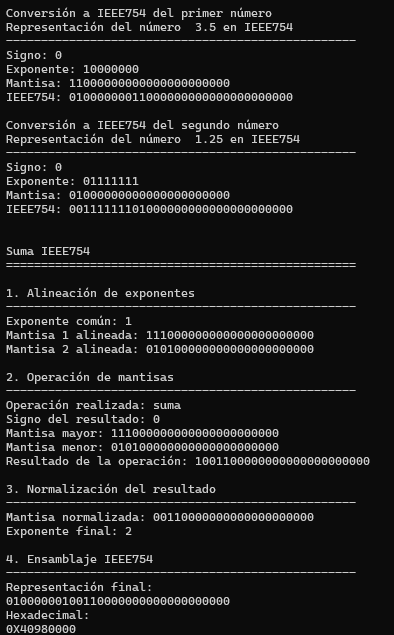
\includegraphics[width=.9\linewidth]{./images/prueba1.png}
\caption{Ejecución del algoritmo para la suma 3.5 + 1.25}
\end{figure}

\begin{figure}[H]
\centering
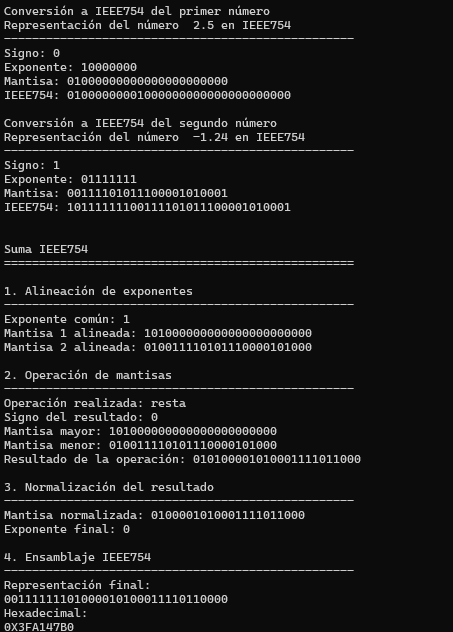
\includegraphics[width=.9\linewidth]{./images/prueba2.png}
\caption{Ejecución del algoritmo para la suma 2.5 + (-1.24)}
\end{figure}

\begin{figure}[H]
\centering
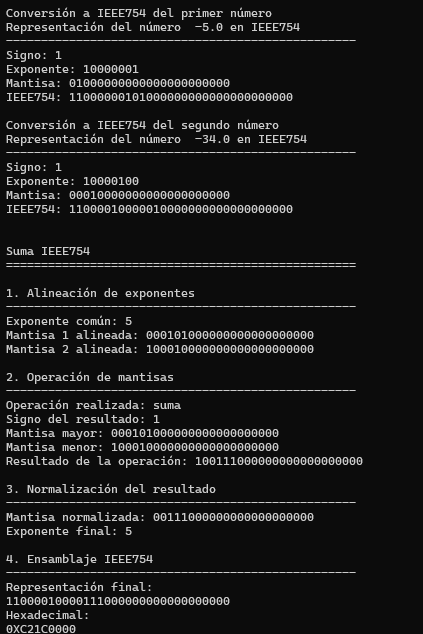
\includegraphics[width=.9\linewidth]{./images/prueba3.png}
\caption{Ejecución del algoritmo para la suma (-5) + (-34)}
\end{figure}

\begin{figure}[H]
\centering
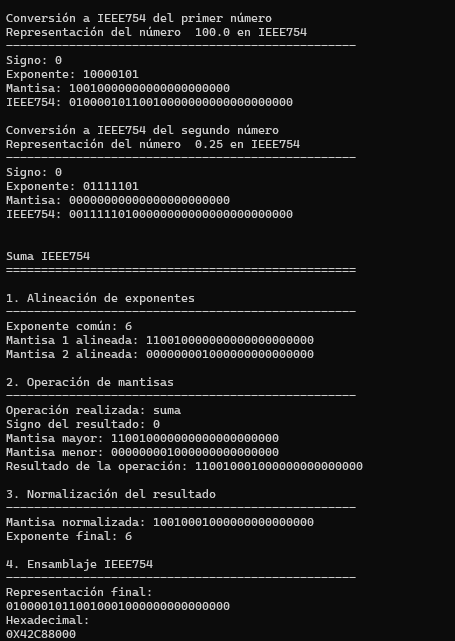
\includegraphics[width=.9\linewidth]{./images/prueba4.png}
\caption{Ejecución del algoritmo para la suma 100 + 0.25}
\end{figure}

\begin{figure}[H]
\centering
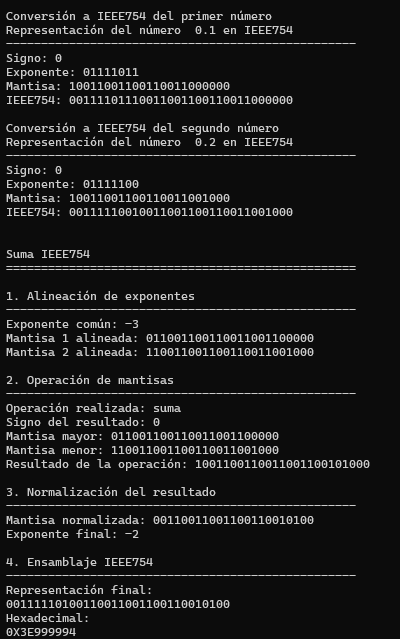
\includegraphics[width=.9\linewidth]{./images/prueba5.png}
\caption{Ejecución del algoritmo para la suma 0.1 + 0.2}
\end{figure}
\section{Conclusiones}
\label{sec:org2bd9ce3}

\begin{itemize}
\item Se implementó satisfactoriamente el algoritmo de suma de números en
formato IEEE754 de precisión simple empleando Python.

\item El desarrollo permitió comprender el funcionamiento interno de una
unidad de punto flotante, especialmente el proceso de alineación de
exponentes, operación entre mantisas y normalización del resultado.

\item La implementación reproduce las principales etapas descritas por el
estándar IEEE754 para la suma en punto flotante.

\item Las pruebas realizadas con números positivos, negativos, enteros y
fraccionarios mostraron resultados consistentes con la representación
IEEE754 de precisión simple.

\item El ejemplo al sumar 0.1 + 0.2 representa los errores que se puede acarrear
al momento de trabajar con números muy pequeños, al obtener un valor un
tanto diferente al 0.3 esperado. Esto sucede ya que el algoritmo trunca los
decimales menos significativos
\end{itemize}
\section{Extra: Ejecución interactiva mediante JavaScript}
\label{sec:org6b629a0}

La implementación principal del algoritmo IEEE754 fue desarrollada en Python.
Sin embargo, debido a que los navegadores no pueden ejecutar directamente
código Python, se desarrolló una versión interactiva utilizando JavaScript,
el cual puede ser interpretado directamente por el navegador.
\section{Referencias}
\label{sec:orgd769abc}

\begin{itemize}
\item IEEE Computer Society. \emph{IEEE Standard for Floating-Point Arithmetic
(IEEE Std 754-2019).} IEEE, 2019.

\item Stallings, William. \emph{Computer Organization and Architecture:
Designing for Performance.} 11th Edition. Pearson.
\end{itemize}
\section{Navegación}
\label{sec:orged40de0}

\href{../index.org}{← Inicio} | \href{../page3-inec.org}{Siguiente: Análisis INEC →}
\end{document}
